\documentclass[a4paper,10pt]{article}

\usepackage{graphicx}
\usepackage[utf8]{inputenc}
\usepackage[T1]{fontenc}
\usepackage{wrapfig}

\usepackage{hyperref}
\setlength{\parindent}{10pt}
\setlength{\parskip}{1.5mm}
\usepackage{geometry}
\geometry{margin=1.25cm}
\addtolength{\textheight}{-1.5cm}
\setlength{\headheight}{32pt}

\usepackage{amsfonts, amstext, color,
	ifthen, fancybox, multirow, fancyhdr, pgf, tikz,%
	colortbl, array, tabularx
}

\definecolor{bgcode}{rgb}{0.95,0.95,0.95}

\usepackage{url}

\usepackage[french]{babel}
\selectlanguage{french}

%partie concernant la gestion des entêtes
\usepackage{fancyhdr}
\pagestyle{fancy}
\usepackage{lastpage}
\renewcommand\headrulewidth{1pt}
\fancyhead[L]{Interface Homme-Machine Android}
\fancyhead[R]{Université de Poitiers}
\renewcommand\footrulewidth{1pt}
\fancyfoot[L]{Département d'Informatique}
\fancyfoot[C]{\textbf{\thepage/\pageref{LastPage}}}
\fancyfoot[R]{année 2021-2022}
%fin

\usepackage{enumitem}

\usepackage{listings}

\usepackage{version}
\usepackage{tcolorbox}

\newcounter{Exercice}
\newcommand{\Exercice}[1]{\refstepcounter{Exercice}%
	\ \vspace{0mm} \\ \hspace{0.8cm}%
	\noindent \hspace*{0.5cm} {\bf Question \theExercice :} #1 \vspace{-13mm} \\ %
	\subparagraph*{}%
}

\lstset{language=Caml,basicstyle=\normalsize\tt,keywordstyle=\ttfamily\bfseries\underbar,%
	commentstyle=\normalsize, extendedchars=true, fontadjust=true, columns = flexible, flexiblecolumns=true,
	linewidth=.975\linewidth, backgroundcolor=\color{bgcode}, frame=tlrb, xleftmargin=1cm}

\lstnewenvironment{ocamlcode}
{\lstset{language=Caml,basicstyle=\normalsize\tt,keywordstyle=\ttfamily\bfseries\underbar,%
		commentstyle=\normalsize, extendedchars=true, fontadjust=true, columns = flexible, flexiblecolumns=true,
		linewidth=.975\linewidth, backgroundcolor=\color{bgcode}, frame=tlrb, xleftmargin=1cm,
		literate={à}{{\`a}}1 {è}{{\`e}}1 {é}{{\'e}}1 {ê}{{\^e}}1,
	}}%, framexleftmargin=5mm,frame=box}}
{}

\lstnewenvironment{fsharp}
{\lstset{language=Caml,basicstyle=\normalsize\tt,keywordstyle=\ttfamily\bfseries\underbar,%
		commentstyle=\normalsize, extendedchars=true, fontadjust=true, columns = flexible, flexiblecolumns=true,
		linewidth=.975\linewidth, backgroundcolor=\color{bgcode}, frame=tlrb, xleftmargin=1cm,
		literate={à}{{\`a}}1 {è}{{\`e}}1 {é}{{\'e}}1 {ê}{{\^e}}1 {ç}{{\c c}}1,
}}%, framexleftmargin=5mm,frame=box}}
{}

\lstnewenvironment{javasansbord}
{\lstset{language=Java,basicstyle=\normalsize\tt,keywordstyle=\ttfamily\bfseries\underbar,%
		commentstyle=\normalsize, extendedchars=true, fontadjust=true, columns = flexible, flexiblecolumns=true,
		linewidth=.975\linewidth,frame=,backgroundcolor=,xleftmargin=0cm,
		literate={à}{{\`a}}1 {è}{{\`e}}1 {é}{{\'e}}1 {ê}{{\^e}}1 {ç}{{\c c}}1,
}}%, framexleftmargin=5mm,frame=box}}
{}

\lstnewenvironment{java}
{\lstset{language=Java,basicstyle=\normalsize\tt,keywordstyle=\ttfamily\bfseries\underbar,%
		commentstyle=\normalsize, extendedchars=true, fontadjust=true, columns = flexible, flexiblecolumns=true,
		linewidth=.975\linewidth, backgroundcolor=\color{bgcode}, frame=tlrb, xleftmargin=1cm,
		literate={à}{{\`a}}1 {è}{{\`e}}1 {é}{{\'e}}1 {ê}{{\^e}}1 {ç}{{\c c}}1,
}}%, framexleftmargin=5mm,frame=box}}
{}

\newboolean{versionenseignant}
%%%%%%%%%%%%%%%%%%%%%%%%%%%%%%%%%%%%%%%%%%%%%%%%%%%%%%%%%%%%%%%%%%%%%%%%%%%%%%%%%%%%%%%%%%%%%%%%%%%%%%%%
%__     __            _
%\ \   / /__ _ __ ___(_) ___  _ __
% \ \ / / _ \ '__/ __| |/ _ \| '_ \
%  \ V /  __/ |  \__ \ | (_) | | | |
%   \_/ \___|_|  |___/_|\___/|_| |_|
% _____                _                         _
%| ____|_ __  ___  ___(_) __ _ _ __   __ _ _ __ | |_
%|  _| | '_ \/ __|/ _ \ |/ _` | '_ \ / _` | '_ \| __|
%| |___| | | \__ \  __/ | (_| | | | | (_| | | | | |_
%|_____|_| |_|___/\___|_|\__, |_| |_|\__,_|_| |_|\__|
%                        |___/ 
%% modifiez le booleen ci-dessous pour generer la version enseignant ou etudiant
%% ===> true = version enseignant
%% ===> false = version etudiant
\setboolean{versionenseignant}{false}
%%%%%%%%%%%%%%%%%%%%%%%%%%%%%%%%%%%%%%%%%%%%%%%%%%%%%%%%%%%%%%%%%%%%%%%%%%%%%%%%%%%%%%%%%%%%%%%%%%%%%%%%
% \includeversion{ensnote}
%\excludeversion{ensnote}
\ifthenelse{\boolean{versionenseignant}}{\includeversion{ensnote}}{\excludeversion{ensnote}}

\tcbuselibrary{breakable}


\newenvironment{solution}%
{\begin{tcolorbox}[breakable,colback=red!5!white,colframe=red!75!black,title=Solution]}%
{\end{tcolorbox}}

%\tcblower

\newenvironment{info}%
{\begin{tcolorbox}[breakable,colback=green!5!white,colframe=green!75!black,title=Information]}%
{\end{tcolorbox}}


\newenvironment{attention}%
{\begin{tcolorbox}[breakable,colback=green!25!white,colframe=red!55!black,title=Attention]}%
{\end{tcolorbox}}


\newenvironment{boxcode}%
{\begin{tcolorbox}[breakable,colback=gray!5!white,colframe=black]}%
	{\end{tcolorbox}}
	
	
\begin{document}
	


\title{\vspace*{-1cm}Réalisation d'un système solaire}
\author{\vspace*{-1.5cm}Interface Homme-Machine: Android
\begin{ensnote}
	(Version enseignant)
\end{ensnote}
}
\date{\vspace*{-1.5cm}version 1}
\maketitle
\thispagestyle{fancy}

Voici les objectifs de ce sujet:
\begin{itemize}
	\item Continuez à manipuler l'IDE \texttt{Unity}.
	\item Création d'un \textit{widget} complexe.
	\item Mécanisme des préfabriqués.
	\item Exportation de son travail: les \textit{unity package}.
\end{itemize}


%\begin{attention}
%	Le sujet ce fait en deux étapes. Avec une proposition notée de votre interface au bout de 2h (si vous avez fini avant la \textit{deadline} rien ne vous empêche de continuer)!
%	
%	N'oubliez pas d'utiliser les bons réflexes de tout développeur:
%	\begin{itemize}
%		\item Le système de log très bien fait sous Android
%		\item Le mode débogue qui vous permet de voir les valeurs des variables pendant 
%	\end{itemize}
%\end{attention}

\section*{Description générale du TP}

La fois précédente, nous avons réalisé notre premier projet Unity et nous avons vu la manipulation de l'interface. La manipulation est simple (mais nécessite quelques calibration). Nous avons réalisé entre autre notre première interface très simplifiée, reposant sur la mécanique des ancres (voire aucune pour certains d'entre vous). La mécanique des ancres n'est pas aisé surtout lorsque les ratio de l'écran peuvent changer (réalisation d'une application PC et une application Android). Ce dernier point ne sera pas étudié dans ce TP car cela rentre dans les aspects très avancées. Cependant, pour le lecteur volontaire ou si vous finissez le TP (donc pas au début) il serait intéressant de regarder ce pointeur \url{https://docs.unity3d.com/2020.1/Documentation/Manual/HOWTO-UIMultiResolution.html}. 

Quoi qu'il arrive, on vous demande dans un premier temps de créer un NOUVEAU projet vide et de fixer une résolution raisonnable\footnote{La résolution que j'ai dans mes versions sont par défaut le \texttt{1024x768}.} de votre Canvas, dans le menu Game de la fenêtre (sinon il s'agit de paramètre spécifique au déploiement de votre application).

\begin{center}
	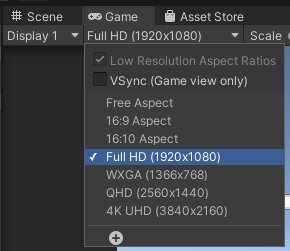
\includegraphics[width=0.5\linewidth]{rc/unity_set_ui_resolution_game}
\end{center}

Une fois réalisez ça, nous pouvons passer à la réalisation de widget complexe. Pour expliquer ce terme, nous allons réalisé un agglomérat de widget existant avec un ou plusieurs scripts pour régir le comportement global du widget.



\section{Premier widget complexe: FormattedInputField}


\section{Widget: SpinnerNumber}


\section{Widget: ComplexSlider}


\section{Exporter son travail}


\section{Toujours plus loin}


\end{document}